
\section{Objetivo}
Que el alumno implemente y refuerce su comprensión del algoritmo A* \par

\section{Introducci\'on}

Resolveremos el problema de navegación en videojuegos con mundos hechos de mosaicos, utilizando el algoritmo A*, siguiendo el ejemplo de Patrick \cite{Lester2003}.

Vamos a asumir que tenemos un personaje que quiere ir desde un punto A hasta un punto B, y que ambos puntos están separados por una pared. Este ejemplo se puede apreciar en la figura~\ref{fig:fig1P4}, donde el cuadrado verde es el punto A, el rojo es el punto B y el rectángulo azul la pared mencionada anteriormente.

\begin{figure}[h!]
  \centering
  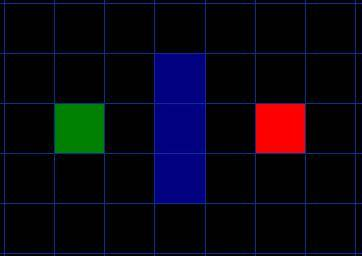
\includegraphics[width=0.4\textwidth]{aestrella/screen1.jpg}
  \caption{Escenario construido con mosaicos discretos. El problema de búsqueda de caminos consiste en encontrar una ruta desde el cuadro verde al cuadro rojo.}
  \label{fig:fig1P4}
\end{figure}

El primer paso que debemos hacer es simplificar el área de búsqueda, dividiendo nuestro mundo en una rejilla cuadrada. Con esto, podremos representar el mundo con una matriz bidimensional. Cada posición en la matriz representará un mosaico del mundo, el cual será transitable o no transitable. Entonces, el objetivo del algoritmo A* es calcular a que mosaico nos debemos mover en cada turno para lograr llegar al punto B. Una vez calculado esto, el personaje del juego se moverá del centro del mosaico donde se ecnuentra actualmente al centro del mosaico obtenido con A*.

A los puntos centrales dentro del mosaico se les llama \classname{nodos}. Esto ya que pudimos haber dividido el mundo en círculos, o en tríangulos. Cada mundo tendrá características diferentes, y se podrá simplificar de distintas formas.

\subsection{Iniciando la b\'usqueda}

Después de haber simplificado el área de búsqueda en nodos, el siguiente paso es dirigir una búsqueda para encontrar el camino más corto. En el algoritmo A*, lo hacemos empezando desde el punto A, comprobando los cuadros adyacentes (estados sucesores) y generalmente buscando hacia fuera hasta que encontremos nuestro destino.

\noindent Empezamos la búsqueda haciendo lo siguiente:

\begin{enumerate}
  \item Empezamos en el punto inicial A y lo añadimos a una \textbf{lista abierta} de cuadrados a tener en cuenta. La lista contiene los cuadrados que podrían formar parte del camino que queremos tomar, pero que quizás no lo hagan. Básicamente, esta es una lista de los cuadrados que necesitan ser considerados.
  \item Nos fijamos en todos los cuadrados alcanzables o transitables adyacentes al punto de inicio, ignorando cuadrados con muros, agua u otros terrenos prohibidos. Se añaden a la lista abierta también. Por cada uno de esos cuadrados, guardamos el punto A como su \textbf{cuadrado padre}. El cuadrado padre es muy importante para trazar nuestro camino.
  \item Sacamos el cuadro inicial A desde la lista abierta y lo añadimos a una \textbf{lista cerrada} de cuadrados que no necesitan ser vistos de nuevo.
\end{enumerate}

En este punto, se tendrá algo como la figura~\ref{fig:fig2P4}. En este diagrama, el cuadrado verde oscuro del centro es el cuadrado de inicio. Está bordeado de azul claro para indicar que el cuadrado ha sido añadido a la lista cerrada. Todos los cuadros adyacentes están ahora en la lista abierta para ser considerados. Cada uno tiene un puntero gris que señala a su padre, el cual es el cuadro inicial.

\begin{figure}[h]
  \centering
  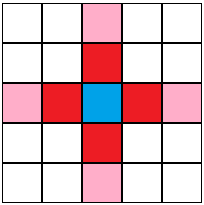
\includegraphics[width=0.3\textwidth]{aestrella/screen2.png}
  \caption{Mosaicos en la lista abierta con referencia a su padre.}
  \label{fig:fig2P4}
\end{figure}


Después, elegimos uno de los cuadrados adyacentes de la lista abierta y más o menos repetimos el proceso anterior. Pero, ¿qué cuadro se debe elegir? Aquel que tenga costo estimado \(f(n)\) más bajo.

\subsection{Puntuando el camino}

La clave para determinar qué cuadrados usaremos para resolver el camino está en la siguiente ecuación:\medskip

\begin{center}
\(f(n) = g(n) + h(n)\)
\end{center}\medskip

donde:

\begin{itemize}
  \item \(g(n)\) es el costo del movimiento para ir desde el punto inicial A a un cierto cuadro de la rejilla (\(n\)), siguiendo el camino generado para llegar ahí.
  \item \(h(n)\) es el costo del movimiento estimado para ir desde ese cuadro de la rejilla (\(n\)) hasta el destino final, el punto B. Esto se conoce como la heurística. Aquí se verá una forma de calcular la heurística, pero no es la única.
\end{itemize}

Nuestro camino se genera al ir repetidamente a través de nuestra lista abierta y eligiendo el cuadrado con la puntuación \(f(n)\) más baja. Este proceso se describirá con más detalle un poco más adelante. Primero veamos más de cerca cómo calculamos esta puntuación.

Tal y como está descrito arriba, \(g(n)\) es el costo del movimiento para ir desde el punto de inicio a un cuadro \(n\) usando el camino generado para llegar ahí. En esta práctica asignaremos un costo de 10 a cada cuadro vertical u horizontal hacia el que nos movamos, y un costo de 14 para un movimiento diagonal. Usamos estos números ya que es más simple poner 14 que \(\sqrt{2}^2\times10\) y porque usar números enteros es mucho más rápido para la computadora. Pronto descubrirás que los algoritmos de búsqueda pueden ser muy lentos si no usas atajos como este.

Ahora que hemos calculado el costo \(g(n)\) mediante un camino específico hasta cierto cuadro, la forma de resolver el costo \(g(n)\) del cuadro es tomar el costo \(g(n)\) de su padre, y luego añadirle 10 o 14 dependiendo de si está en diagonal u ortogonal con respecto al cuadro padre.

\(h(n)\) puede ser estimado de diferentes maneras. El método que usaremos aquí se llama el método Manhattan, donde se calcula el número total de cuadros movidos horizontalmente y verticalmente para alcanzar el cuadrado destino desde el cuadro actual, sin hacer uso de movimientos diagonales e ignorando cualquier obstáculo. Luego multiplicamos el total por 10. Se llama método Manhattan porque es como calcular el número de manzanas que hay desde un lugar a otro, donde no puedes acortar atravesando en diagonal una manzana. Es una estimación de la distancia que queda, no de la distancia actual, es por eso que se llama heurística.

\(f(n)\) se calcula sumando \(g(n)\) y \(h(n)\). El resultado del primer paso en nuestra búsqueda puede verse en la figura~\ref{fig:fig3P4}. Las puntuaciones \(f(n)\), \(g(n)\) y \(h(n)\) están escritas en cada cuadrado. En el cuadro inmediatamente a la derecha del cuadro inicial, se escribieron las letras F, G y H para indicar dónde se encuentran los valores de \(f(n)\), \(g(n)\) y \(h(n)\).

\begin{figure}[h!]
  \centering
  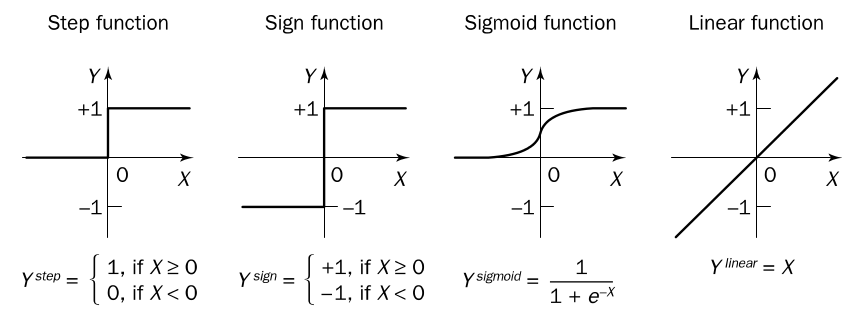
\includegraphics[width=0.5\textwidth]{aestrella/screen3.png}
  \caption{Cálculo de \(f\),\(g\) y \(h\) que se agregan a la lista abierta.}
  \label{fig:fig3P4}
\end{figure}

Así pues, obsevaremos algunos ejemplos de estos cuadros. En el cuadrado con letras, \(g(n)=10\). Esto es debido a que está solo a un cuadro del cuadrado inicial en dirección horizontal. Los cuadrados inmediatamente encima, abajo y a la izquierda del cuadrado inicial; tienen todos el mismo valor \(g(n)\) de 10. Los cuadros diagonales tienen un valor \(g(n)\) de 14.

Las puntuaciones \(h(n)\) se calculan estimando la distancia Manhattan hasta el cuadrado rojo objetivo, moviéndose solo horizontal y verticalmente e ignorando el muro que está en el camino. Usando este método, el cuadro a la derecha del inicial, está a 3 cuadros del cuadrado rojo con una puntuación \(h(n)\) de 30. El cuadrado está a sólo 4 cuadros de distancia (recuerda que solo nos movemos en dirección horizontal y vertical) con una puntuación \(h(n)\) de 40. Probablemente podrás calcular las puntuaciones \(h(n)\) para los demás cuadros.


\subsection{Continuando la b\'usqueda}

Para continuar la búsqueda, simplemente elegimos la puntuación \(f(n)\) más baja de todos aquellos que estén en la lista abierta. Para que esta operación se realize lo más eficientemente posible, la lista abierta se implementará con una cola de prioridades. Después hacemos lo siguiente con el cuadro seleccionado:

\begin{enumerate}
  \item Lo sacamos de la lista abierta y lo añadimos a la lista cerrada.  

  \item Comprobamos todos los cuadrados adyacentes, ignorando aquellos que estén en la lista cerrada o que sean intransitables: terrenos con muros, agua o cualquier terreno prohibido; añadimos los cuadros a la lista abierta si no están ya en esa lista. Hacemos que el cuadro seleccionado sea el \textbf{padre} de los cuadros nuevos.

  \item Si el cuadro adyacente ya está en la lista abierta, comprobamos si el camino nuevo a ese cuadro es mejor que el que tenía, es decir, si el valor de \(g(n)\) con este padre es menor que el que se había estimado con su padre anterior. Si no es así, no haremos nada. Por otro lado, si el costo \(g(n)\) del nuevo camino es más bajo, cambiamos el padre del cuadro adyacente al cuadro seleccionado (en el diagrama superior, cambia la dirección del puntero para que señale al cuadro seleccionado). Finalmente, recalculamos \(f(n)\) y \(g(n)\) de ese cuadrado.
\end{enumerate}


\section{Desarrollo e implementaci\'on}

La práctica consiste en implementar el algoritmo A* y generar una visualización de éste resolviendo un problema. Ustedes pueden modificar el mundo del problema, para que puedan ver cómo se comporta A* con distintas localizaciones de obstáculos y de nodos de inicio y fin. 


\subsection{Implementaci\'on}


Se debe programar lo referente al algoritmo A* y la función heurística.
También necesitarán implementar sus listas abierta y cerrada (o usar alguna biblioteca o clase ya implementada de \classname{Java}).
Se volverá a trabajar con \classname{Processing}.

\noindent Los métodos que deberán implementar son los siguientes:

\begin{enumerate}
  \item \classname{calculaHeuristica(Mosaico meta)}
  \item \classname{expandeNodoSiguiente()}
\end{enumerate}

\noindent Cada método se encuentra especificado dentro del archivo \classname{AEstrella.java}.


\section{Requisitos y resultados}

Para evaluar y calificar la práctica es necesario que se implementen todos los métodos mencionados e indicados en el código, respetando implementar sólo lo que se pide (para evitar comportamientos extraños de la simulación).
Es completamente válido utilizar bibliotecas adicionales si lo consideran necesario, así como la creación y uso de sus propios métodos auxiliares si lo desean.

Si crean métodos auxiliares, no olviden documentar cual es su función.


%  \begin{thebibliography}{1}

%   \bibitem{notes} Patrick Lester {\em A* Pathfinding para Principiantes}  2003 :
%   http://www.policyalmanac.org/games/articulo1.htm .

% \end{thebibliography}
